\documentclass{article}

\usepackage[utf8]{inputenc}
\usepackage[pdftex]{graphicx}
\usepackage[left=3cm,right=3cm,top=3cm,bottom=3cm]{geometry}
\usepackage[T1]{fontenc}
\usepackage[francais,english]{babel}
\frenchbsetup{StandardLists=true}
\selectlanguage{english}


\usepackage{amsmath}
\usepackage{amssymb}
\usepackage{mathtools}

\usepackage{caption}
\usepackage[hidelinks]{hyperref}
\usepackage{xcolor}

\usepackage{listings}

\usepackage{graphicx}

\renewcommand\thesection{\arabic{section}}

\usepackage{fancyhdr}
\pagestyle{fancy}
\fancyhf{}
\fancyhead[R]{\thepage}


\title{[INFO-F409] Learning Dynamics \\ First assignment}
\author{\bsc{BUI QUANG PHUONG} Quang Linh \\ Université libre de Bruxelles - ULB ID : 000427796  \\ MA1 Computer Sciences}
\date{November 2018}

\begin{document}

\maketitle

\section{The Hawk-Dove game}

\subsection*{Conventions and notations}
First of all, the Hawk-Dove game is modeled by the matrix presented in the \autoref{table:payoffMatrix}. 

\begin{center}
\begin{tabular}{|l|r|r|}
  \hline
  			   & Hawk & Dove \\
  \hline
  		   & \hspace{1cm} $\frac{V-D}{2}$ & 0 \\
  	Hawk &	\multicolumn{1}{|l|}{$\frac{V-D}{2}$}		& 	\multicolumn{1}{|l|}{$V$ }		\\
  \hline
    		   & \multicolumn{1}{|r|}{$V$} & \hspace{1cm} $\frac{V}{2}-T$  \\
  Dove &	\multicolumn{1}{|l|}{0}		& 	\multicolumn{1}{|l|}{$\frac{V}{2}-T$}		\\
  \hline
\end{tabular}
\captionof{table}{Payoff matrix of the Hawk-Dove game}
\label{table:payoffMatrix}
\end{center}

The different actions of a player $i \in \{1,2\}$ are denoted by the set $\mathcal{A} = \{H,D\}$ where $H$ is the hawk action and  
$D$ the dove action. Moreover, to denote the different actions payoff, we need an utility function of those actions. This utility function is then written  : 
$$ u_{i}(a_{i}, a_{-i}) $$ such that $a_{i}$ is an action of player $i$ and $a_{-i}$ is the action of the other player where player $i$ choses $a_{i}$. For instance,  $ u_{1}(Hawk, Dove) = V $ and $ u_{2}(Hawk, Dove) = 0 $). \\

In the case of mixed strategies, the notion of \textbf{expected value} of a payoff function is used and is written in the general case :
$$ U_{i}(p_{1}, ... , p_{k }) = p_{k} u(a_{k})$$ where $i$ is a player, $p_{k}$ is the probability that the other player chose the action $a_{k}$. 
In the case of the Hawk-Dove game, the expected value formula would be written such that $k=2$ because it exists only 2 actions, i.e. :  $$ U_{i}(p_{1}, p_{2}) = p_{1} u(a_{1}) + p_{2} u(a_{2})$$

Furthermore, to find Nash equilibria, best responses have to be found. Those one will be highlighted in \colorbox{pink}{red} for the line player considered as player one and \colorbox{green}{green} for the column player considered as player two. 

\subsection{Question 1 - Nash equilibrium}

\subsubsection*{Statement} 
\noindent
\textit{ Find all the (mixed strategy) Nash equilibria of this game. How do the results change when the order of the parameters V, D and T is changed (V>D, D>T, etc.)?}

\subsubsection*{Sign of V, D and T} 
Before starting the analysis, we should remind that $V$ and $D$ are representing respectively the fitness value of winning resources in fight and costs of injury thereby it would not make sense having negative values. $V$ and $D$ are then always positive values. Same for $T$ which is the cost of wasting time. The time wasted is obviously always a positive value. To summarize, 
$$ V, D, T \ge 0 $$  


\subsubsection{First case : $V>D$} 

In the first case, we consider that $V>D$. Therefore, we know that the value of $u_{i}(Hawk, Hawk) = \frac{V-D}{2}$ will be strictly positive. In this case, the choice of both players are quiet easy. As illustrated in \autoref{table:NE-case1}, the Nash equilibrium is $(Hawk, Hawk) \in \mathcal{A}$. Indeed, both players are chosing $Hawk$ because if one of them is switching to $Dove$ then $u_{i}(Hawk,Hawk)$ which was a positive value becomes $u_{1}(Dove,Hawk)$ for player 1 or $u_{2}(Hawk,Dove)$ for player 2 which equals zero. Thus, they obviously prefer to pick $(Hawk,Hawk)$. \\

\begin{center}
\fbox{Nash equilibrium when $(V>D) = \{(Hawk, Hawk)\}$}
\end{center} 

\begin{center}
\begin{tabular}{|l|r|r|}
  \hline
  			   & Hawk & Dove \\
  \hline
  		   & \hspace{1cm} \colorbox{green}{$\frac{V-D}{2}>0$} & 0 \\
  	Hawk &	\multicolumn{1}{|l|}{\colorbox{pink}{$\frac{V-D}{2}>0$}}		& 	\multicolumn{1}{|l|}{\colorbox{pink}{$V$}}		\\
  \hline
    		   & \multicolumn{1}{|r|}{\colorbox{green}{$V$}} & \hspace{1cm} $\frac{V}{2}-T$  \\
  Dove &	\multicolumn{1}{|l|}{0}		& 	\multicolumn{1}{|l|}{$\frac{V}{2}-T$}		\\
  \hline
\end{tabular}
\captionof{table}{Nash equilibrium/Best responses in case 1}
\label{table:NE-case1}
\end{center}

\subsubsection{Second case : $V=D$}
The second case considers the same value for $V$ and $D$ which means that $\frac{V-D}{2} = 0$. The \autoref{table:NE-case2} shows the Nash equilibria for that case. We can see that there doesn't exist only one Nash equilibrium, but three. $(Hawk,Hawk)$ stays a Nash equilibrium in this case, but $(Dove,Hawk)$ and $(Hawk,Dove)$ are now also Nash equilibria. In other words, if player 2 is chosing $Hawk$, the best response to it is whether $(Hawk,Hawk)$ or $(Dove,Hawk)$ because $u_{1}(Hawk,Hawk)=u_{1}(Dove,Hawk)=0$. On the other hand, if player 2 is chosing $Dove$, the best response is only $(Hawk,Dove)$ since $u_{1}(Hawk,Dove)>u_{1}(Dove,Dove) \equiv V > \frac{V}{2}-T$. By symmetry, it is also valid for the opposite case where player 1's choice is known, so that the best  responses are (symmetrically) equivalent which means $(Hawk,Hawk)$,$(Hawk,Dove)$ and $(Dove, Hawk)$ are the best responses for player 2. \\

\begin{center}
\fbox{Nash equilibria when $(V=D) = \{(Hawk, Hawk) , (Hawk,Dove) , (Dove,Hawk)\}$} 
\end{center}

\begin{center}
\begin{tabular}{|l|r|r|}
  \hline
  			   & Hawk & Dove \\
  \hline
  		   & \hspace{1cm} \colorbox{green}{$\frac{V-D}{2}=0$} & \colorbox{green}{0} \\
  	Hawk &	\multicolumn{1}{|l|}{\colorbox{pink}{$\frac{V-D}{2}=0$}}		& 	\multicolumn{1}{|l|}{\colorbox{pink}{$V$}}		\\
  \hline
    		   & \multicolumn{1}{|r|}{\colorbox{green}{$V$}} & \hspace{1cm} $\frac{V}{2}-T$  \\
  Dove &	\multicolumn{1}{|l|}{\colorbox{pink}{0}}		& 	\multicolumn{1}{|l|}{$\frac{V}{2}-T$}		\\
  \hline
\end{tabular}
\captionof{table}{Nash equilibria/Best responses in case 2}
\label{table:NE-case2}
\end{center}

\subsubsection{Third case : $V<D$}
Finally, we are now considering that $V<D$. Therefore, $u_{i}(Hawk, Hawk) = \frac{V-D}{2}$ is now strictly a negative value. 
The \autoref{table:NE-case3} is showing the Nash equilibria for this case. Compared to the previous case, $(Hawk,Hawk)$ is not a Nash equilibrium anymore but $(Hawk,Dove)$ and $(Dove,Hawk)$ keep there. Indeed, when player 2 is playing $Hawk$, player 1 would play $Dove$ since $u_{1}(Hawk, Hawk) < u_{1}(Dove, Hawk) \equiv \frac{V-D}{2} < 0$. In the case where player 2 is playing $Dove$, it doesn't change, it means that  $u_{1}(Hawk, Dove) = V$ is still greater than $u_{1}(Dove, Dove) = \frac{V}{2}-T$. As reasoned in the previous case, this is also valid when player 2 is depending of player 1's choice thanks to the matrix's symmetry. \\

\begin{center}
\fbox{Nash equilibria when $(V<D) = \{(Hawk,Dove), (Dove,Hawk)\}$} 
\end{center}

\begin{center}
\begin{tabular}{|l|r|r|}
  \hline
  			   & Hawk & Dove \\
  \hline
  		   & \hspace{1cm} $\frac{V-D}{2}<0$ & \colorbox{green}{0} \\
  	Hawk &	\multicolumn{1}{|l|}{$\frac{V-D}{2}<0$}		& 	\multicolumn{1}{|l|}{\colorbox{pink}{$V$}}		\\
  \hline
    		   & \multicolumn{1}{|r|}{\colorbox{green}{$V$}} & \hspace{1cm} $\frac{V}{2}-T$  \\
  Dove &	\multicolumn{1}{|l|}{\colorbox{pink}{0}}		& 	\multicolumn{1}{|l|}{$\frac{V}{2}-T$}		\\
  \hline
\end{tabular}
\captionof{table}{Nash equilibria/Best responses in case 3}
\label{table:NE-case3}
\end{center}

\subsubsection{What about the value of $T$ ?}
As you can see, the different cases are not depending of the value of $T$. In each case, $(Dove, Dove)$ will never be a Nash equilibrium since that $\frac{V}{2}-T$ will always be smaller than $V$ (as reminder, $V$ and $T > 0$), then $(Dove,Dove)$ will never be the best response.  

\subsubsection{Mixed strategy}
To find the mixed strategy Nash equilibrium, we have to take into account the probabilities $p$ and $q$ which are respectively the probabilities of playing a certain action for player 1 and player 2. The general probabilities of a 2x2 game's matrix is shown in the \autoref{fig:proba-2x2}. 

\begin{figure}[h]
  \centering
  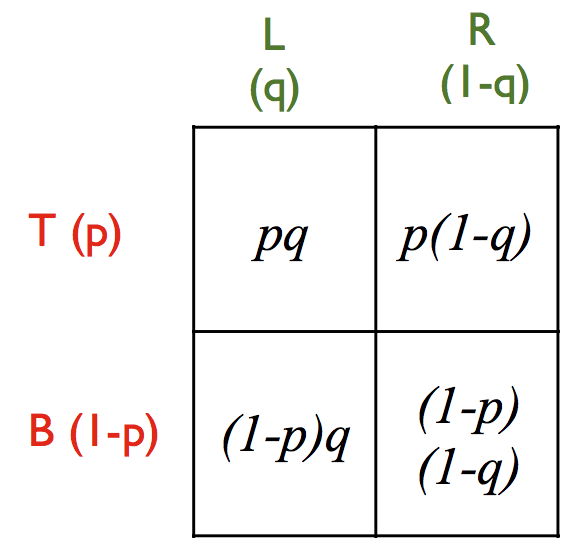
\includegraphics[scale=0.35]{figures/proba-2x2.png}
  \caption{Probabilities of a 2x2 game's matrix}
  \label{fig:proba-2x2}
\end{figure}

Thus, we have to compute the expected value of each case which means the player 1’s expected payoff for the pure strategy $Hawk(p)$ and $Dove(1-p)$, same for player 2 i.e $Hawk(q)$ and $Dove(1-q)$.

Therefore, for player 1 we obtain those equations \footnote{$U_{i}^{j}$ means the player $i$’s expected payoff for the
pure strategy $j$} : 

\begin{flalign}
 U_{1}^{H} &= q \cdot (\frac{V-D}{2}) + (1-q) \cdot V  \\
 U_{1}^{D} &= (1-q) \cdot (\frac{V}{2} - T) 
\end{flalign}

To find the value of probability $q$, we equalize the two equations to isolate $q$ : 
\begin{flalign}
 q \cdot (\frac{V-D}{2}) + (1-q) \cdot V &= (1-q) \cdot (\frac{V}{2} - T)  \\
 \frac{qV}{2} - \frac{qD}{2} + V - pV &= \frac{V}{2} - T - \frac{qV}{2} + qT \nonumber \\
 - \frac{qD}{2} &= - \frac{V}{2} - T + pT \nonumber \\ 
 \frac{qD}{2} + pT &= \frac{V}{2} + T \nonumber \\ 
 q \cdot (\frac{D}{2} + T) &= \frac{V}{2} + T \nonumber \\
 q  &= \frac{\frac{V}{2} +  T}{\frac{D}{2} + T} \nonumber \\  
 \Aboxed{q &= \frac{V+2T}{D+2T}}
\end{flalign}

By symmetry, we can deduct the equations for player 2 :  
\begin{flalign}
 U_{2}^{H} &= p \cdot (\frac{V-D}{2}) + (1-p) \cdot V  \\
 U_{2}^{D} &= (1-p) \cdot (\frac{V}{2} - T) 
\end{flalign}

therefore, the value of $p$ will be the same as $q$ too : 
\begin{flalign}
p &= \frac{V+2T}{D+2T}
\end{flalign}

which means that : 
\begin{flalign}
p = q = \frac{V+2T}{D+2T}
\end{flalign}


\subsection{Question 2 - Mixed strategy drawing}
% a faire demain (au brouillon)

\subsubsection*{Statement}

\textit{Under which conditions does displaying become more beneficial than escalating? Draw the set of all mixed strategies.} 

\section{Which social dilemma ?}

%commencer à lire les slides sur ça demain

\section{Games in finite population}


\end{document}